\chapter{Development of Hybrid Targets}
\label{chap4}

\section{Overview}

In the first part of this chapter, I present the development of high-performance polarized $^{3}$He targets for use in electron scattering experiments that utilize the technique of alkali-hybrid spin-exchange optical pumping. Data of 24 separate target cells are presented, each of these cells was constructed while preparing of one of four experiments at Jefferson Laboratory. The results document dramatic improvement in the performance of polarized $^{3}$He targets. I focus on the data analysis work in this chapter since most of the data had already been taken by the time I joined the group. Other details are described by Jaideep Singh~\cite{PhysRevC.91.055205}. With the wide range of data, we successfully determined the so-called X-factors that quantify a temperature-dependent and as-yet poorly understood spin-relaxation mechanism that limits the maximum achievable $^{3}$He polarization to well under 100\%. We developed a simulation of the alkali-hybrid spin-exchange optical pumping process that provided a means to calculate volume averaged alkali polarization. The data collected also served as a measurement of the K-$^{3}$He spin-exchange rate coefficient $k_{se}^{K}=(7.46\pm0.62)\times10^{-20}$ cm$^{3}$/s over the temperature range 503 K to 563 K.

In the second part of the chapter, I report the results we have so far on developing the next generation target cell. As mentioned in previous chapters, target cells are composed of two distinct chambers: a pumping chamber (PC) where gas is polarized, and a target chamber through which the electron beam passes. The two chambers are traditionally connected by a single transfer tube. The polarization in the target chamber is replenished by gas from pumping chamber through diffusion. This is not a problem as long as the time scales associated with diffusion are short compared with the time scales associated with the depolarization process. The time scale of diffusion through transfer tube is roughly 0.5-1 hour. Due to the increasing electron beam current, the polarization gradient between the two chambers increased from 1-2\% to up about 8\% in more recent experiments. Future experiments are likely to use beam currents 4 times or more of what caused 8\% polarization gradient. A new design was developed Peter Dolph which circulates the gas with convection instead of diffusion. Dolph demonstrated the design with a prototype cell, later I tested the first and second convection style cells with high $^{3}$He polarization while having convection on. The success with our new design enables future experiment to run with higher electron beam current without causing too much polarization gradient.

\section{Development of Targets without Convection}

Spin-exchange optical pumping (SEOP) is a two step process in which an alkali-metal vapor is polarized with optical pumping which subsequently polarizes noble-gas nuclei via spin-exchange collisions. A pure Rb vapor was used to polarize $^{3}$He prior to the development of hybrid cells. However, it was found that K is far more efficient than Rb at transferring its polarization to $^{3}$He nuclei. Hybrid mixtures of Rb and K were used more and more frequently to improve the efficiency of the polarization process. In alkali-hybrid spin-exchange optical pumping (AHSEOP), the Rb vapor is polarized by circularly polarized laser, but the polarization of Rb valence electrons is then rapidly shared with the K. The rate at which Rb and K exchange polarization is so fast that their polarizations can be thought of as being equal. If the alkali-hybrid mixture contains significantly more K than Rb with appropriate ratio, the spin-exchange efficiency is greatly improved so that the rate at which $^{3}$He is polarized is increased significantly for a given amount of laser power.

The second factor that proved to have improved target cells performance greatly was the use of spectrally-narrowed diode lasers. We were able to achieve higher alkali polarization with the aid of these lasers, which in turn reduced the required laser power. The origins of the improved cell performance are twofold. Firstly, these narrowband lasers have spectral profiles closely match the Rb D$_{1}$ absorption line shapes, which results in higher optical pumping rates and hence higher alkali polarizations. Secondly, it allows us to use higher alkali densities (which increases spin-exchange rates) without sacrificing alkali polarization. 

The data collected over the years include $^{3}$H polarization achieved under different operating conditions, the time constants of polarization process, the geometric properties of the target cells, and cell fill information such as pressure and ratio of K to Rb in hybrid mixtures, the time constants of spin relaxation process. In roughly half the cells, the alkali polarization and alkali density were also measured with Faraday Rotation techniques. The results contain several thousand hours worth of data and provide valuable information for future cell development.

Two figures of merit (FOMs) are plotted in Fig.~\ref{fig:foms}, both of which are relevant in evaluating the performance of a polarized $^{3}$He target. The one on the left axis is the effective luminosity $\mathcal{L}^{eff}=\mathcal{L}P_{He}^{2}$, where $\mathcal{L}$ is the luminosity for a fixed-target experiment (the product of beam current, target density, and interaction length) and $P_{He}$ is the $^{3}$He polarization. The luminosity $\mathcal{L}$ represents the number of scattering opportunities per unit time per unit area, while $P_{He}^{2}$ accounts for the reduction in statistical error of some polarization-dependant asymmetry. The FOM on the right axis is used to quantify the potential effective luminosity of a target. The definition is $\mathcal{L}^{N}=\mathcal{N}\Gamma_{s}P_{He}^{2}$, where $\mathcal{N}$ is the total number of $^{3}$He atoms in the target, $\Gamma_{s}$ is the rate at which polarization builds up. The target cell Antoinette is the first one with such high value of $\mathcal{L}^{N}$, which indicates tis cell could tolerate higher luminosities than previously achieved. The high potential further demonstrates the importance of the development of the new convection style target cell. With even higher luminosities in electron scattering experiments, significantly faster gas transfer becomes quite necessary to reduce the polarization gradient between the pumping chamber of target chamber.

\begin{figure}[t!]
	\centering
	\resizebox{0.91\textwidth}{!}{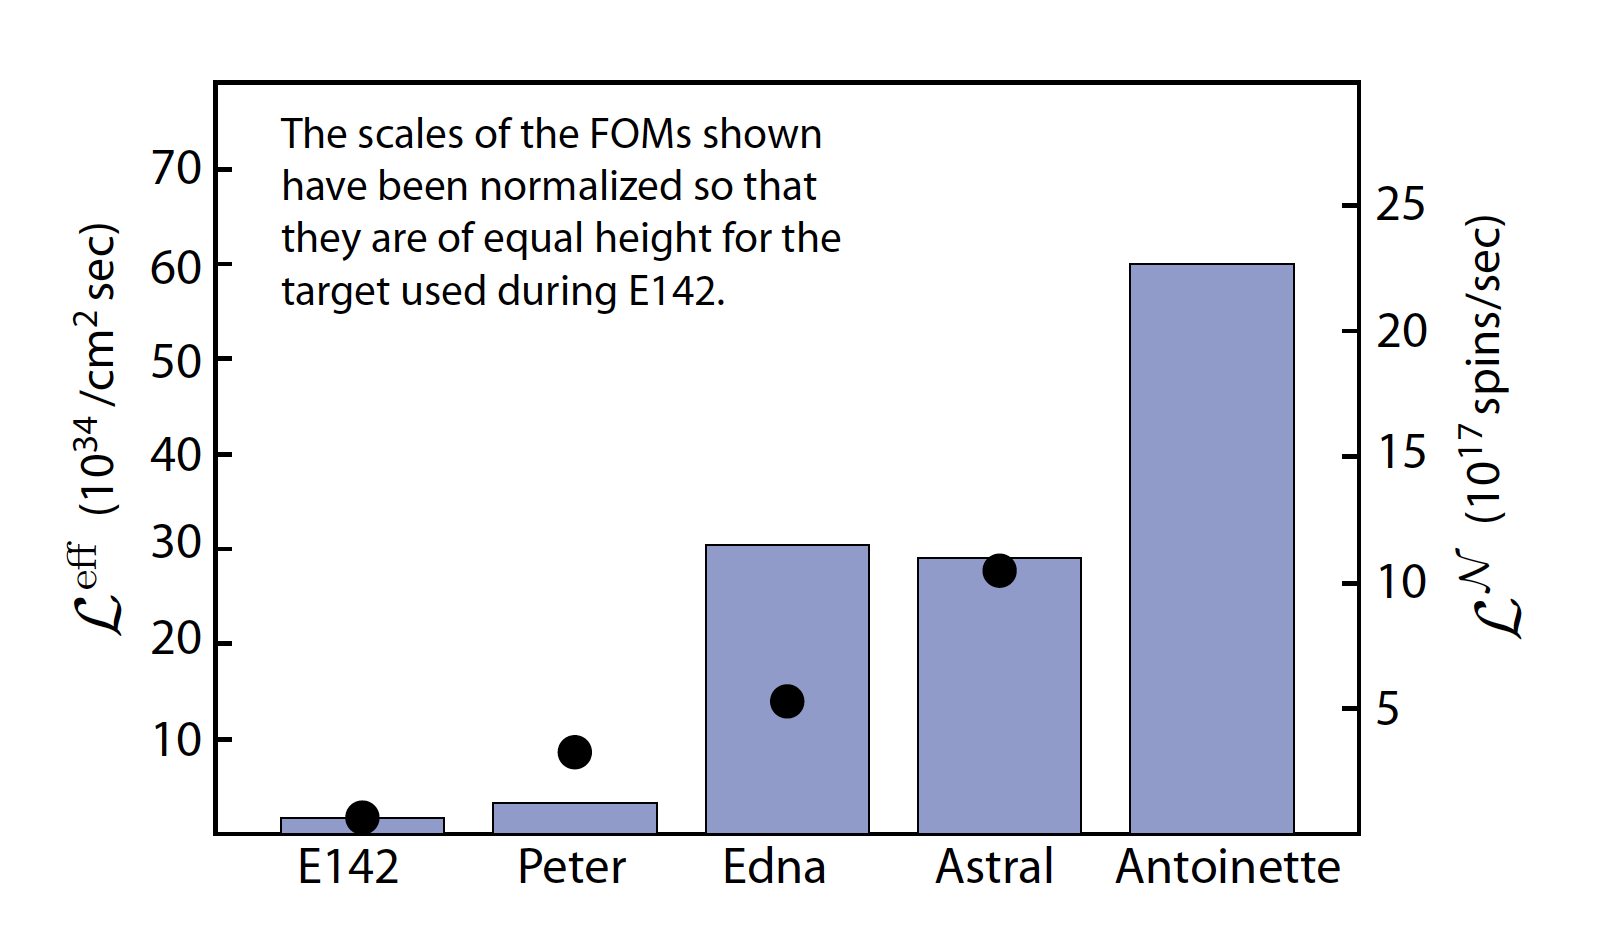
\includegraphics{target_performance.png}}
	\caption{{Shown are two figures of merit (FOM) for targets built for the indicated experiments.  The circles (left axis) indicate the number of spins being polarized per second weighted by the square of polarization.  The bars (right axis) represent the luminosity weighted by the square of polarization.  While the first FOM is an indication of the potential of the polarization technique, the second FOM indicates performance achieved during an experiment.  The actual cells used to formulate the FOMs are not necessarily the same.}}
	\label{fig:foms}
\end{figure}

\subsection{Experimental Methods}





